\begin{figure}[tbp]
\centering
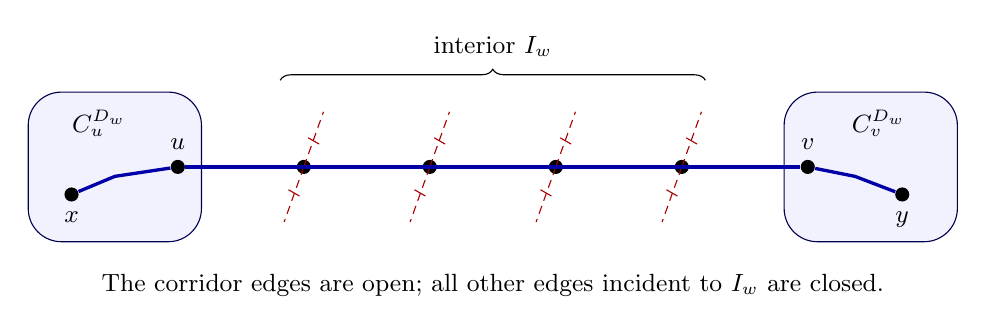
\begin{tikzpicture}[x=1cm,y=1cm,font=\small,
  dot/.style={circle,fill,inner sep=1.8pt},
  open/.style={very thick,blue!65!black},
  closed/.style={densely dashed,red!65!black}]
\fill[blue!5,rounded corners=12pt] (-1.9,-.95) rectangle (.3,.95);
\draw[blue!30!black,rounded corners=12pt] (-1.9,-.95) rectangle (.3,.95);
\fill[blue!5,rounded corners=12pt] (7.7,-.95) rectangle (9.9,.95);
\draw[blue!30!black,rounded corners=12pt] (7.7,-.95) rectangle (9.9,.95);
\node at (-1,.55) {$C_u^{D_w}$};
\node at (8.9,.55) {$C_v^{D_w}$};
\node[dot,label=below:$x$] (x) at (-1.35,-.35) {};
\node[dot,label=above:$u$] (u) at (0,0) {};
\node[dot,label=above:$v$] (v) at (8,0) {};
\node[dot,label=below:$y$] (y) at (9.2,-.35) {};
\draw[open] (x)--(-.8,-.12)--(u);
\draw[open] (v)--(8.6,-.12)--(y);
\foreach \q in {1.6,3.2,4.8,6.4}{
  \node[dot] at (\q,0) {};
  \draw[closed] (\q,0)--(\q+.25,.7);
  \draw[closed] (\q,0)--(\q-.25,-.7);
  \draw[red!65!black] (\q+.055,.37)--(\q+.195,.29);
  \draw[red!65!black] (\q-.195,-.29)--(\q-.055,-.37);
}
\draw[open] (u)--(v);
\draw[decorate,decoration={brace,amplitude=4pt}] (1.3,1.1)--(6.7,1.1)
  node[midway,above=5pt] {interior $I_w$};
\node[align=center,text width=10.5cm] at (4,-1.5)
{The corridor edges are open; all other edges incident to $I_w$ are closed.};
\end{tikzpicture}
\caption{A forced corridor and its two exterior legs. On the event that
the entire corridor is pivotal for $x\leftrightarrow y$, its endpoints
belong to distinct clusters in $D_w=V\setminus I_w$. The event $Q_w$
fixes only bits incident to $I_w$ and is independent of the exterior
percolation.
Dashed stubs represent closed blocker edges; they are schematic.}
\label{fig:corridor}
\end{figure}
